\chapter{Les lignes de transmission}

\section{Résultat numérique}
\begin{wrapfigure}[13]{l}{4.5cm}
	\vspace{-5mm}
	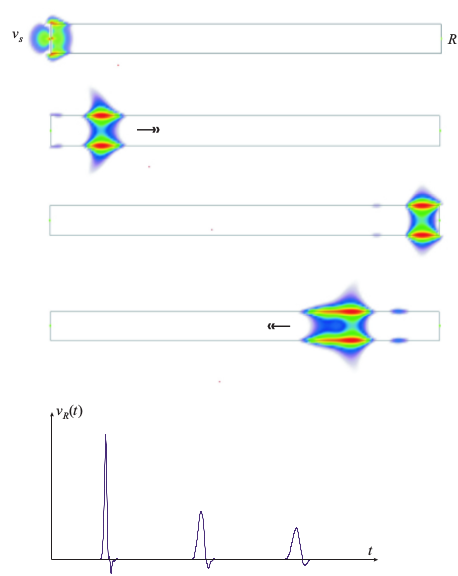
\includegraphics[scale=0.25]{ch2/image1.png}
	\captionof{figure}{ }
\end{wrapfigure}
Considérons un circuit composé uniquement d'une source de tension $s$ et d'une résistance $R$. Dans 
l'approximation quasi-statique
\begin{equation}
v_R(t) = v_s(t)
\end{equation}
Sortons de cette approximation et considérons que la tension de la source est gaussienne. Ci-dessous, 
coloré, la norme de la composante verticale du champ électrique. La ou il est non-nul, une ddp 
se crée : une \textit{onde de tension} se propage. Après $R$, une partie est \textit{réfléchie} vers 
la source. Elle peut ainsi faire plusieurs aller-retours. La \textbf{ligne de transmission} relie 
la source à la charge. Ce vocable est utilisé lorsque l'approximation quasi-statique ne s'applique 
plus. Trois types de lignes différentes sont représentées ci-dessous.
\begin{center}
	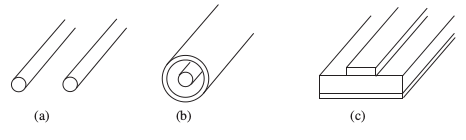
\includegraphics[scale=0.45]{ch2/image2.png}
	\captionof{figure}{(a) Ligne bifilaire (b) ligne coaxiale (c) ligne micro-ruban (microstrip). 
	Notons que l'on désigne le \textit{plan de masse} la ligne du dessous.}
\end{center}

\section{Propagation sur une ligne infinie}
La ligne infinie permet de se débarrasser des "aller-retours". Considérons une source "continue" 
de type créneau. La nouveauté est que l'on considère ici les fils : nous avons vu que la ddp entre 
ceux-ci dépend de la position et du temps : $v=v(z,t)$.\\
Considérons une source idéale $v_s$. Avant enclenchement, la ligne est neutre. Une fois celle-ci 
allumée, sous l'effet d'un champ électrique, il apparaît des densités de charges induites 
créant une ddp $v_s$. Ces charges induites provoquent l'apparition d'un champ électrique un peu 
plus loin sur la ligne : ce dernier se propage sans être atténué. Le signal n'est donc pas donné 
par le mouvement des $e^-$ (qui eux sont "plaqués" à l'extérieur de la ligne) mais par le déplacement 
du champ électrique. La ligne sert ainsi de \textit{guide} pour le champ électrique par apparition 
de charges induites.\newpage


\begin{wrapfigure}[15]{l}{5.5cm}
%	\vspace{-5mm}
	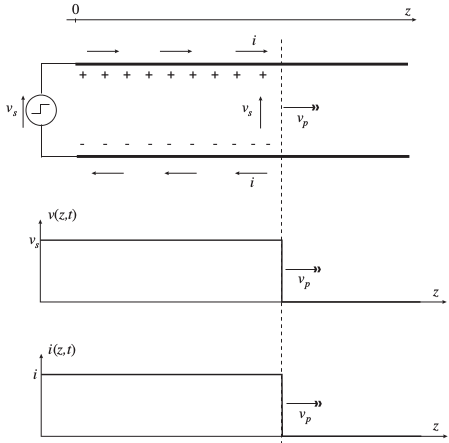
\includegraphics[scale=0.35]{ch2/image3.png}
	\captionof{figure}{ }
\end{wrapfigure}
Cette ddp $v(z,t)$ est liée à la densité de charge induite $q_l(z,t)$ par la capacité linéique de 
la ligne $C_1$
\begin{equation}
v(z,t) = \dfrac{q_l(z,t)}{C_1}
\label{eq:LienCapa}
\end{equation}
En tenant compte du délai de propagation
\begin{equation}
v(z,t) = v_s(t-z/v_p)
\end{equation}
où $v_p$ est la vitesse de propagation (inconnue). On en tire
\begin{equation}
\dfrac{\partial v}{\partial z} = -\dfrac{1}{v_p}\dfrac{\partial v}{\partial t}
\label{eq:ASat}
\end{equation}
La densité de charge induite est nulle lorsque 
le front d'onde n'est pas passé et vaut $v_sC_1$ là où il est déjà passé : la ligne se charge. Là 
où le front d'onde est passé, les $e^-$ ont subi un déplacement microscopique formant un champ qui 
lui-même, crée un courant : \textit{onde de courant}. Celle-ci doit satisfaire
\begin{equation}
\dfrac{\partial i}{\partial z} = -\dfrac{1}{v_p}\dfrac{\partial i}{\partial t}
\end{equation}
Avec cette relation et la conservation de la charge $\displaystyle\dfrac{\partial i}{\partial z} 
=-\dfrac{\partial q_l}{\partial t}$ on obtient après intégration (charge initiale et courant 
initial nuls $\forall z$)
\begin{equation}
i(z,t) = v_pq_l(z,t)
\end{equation}
En utilisant cette relation et \autoref{eq:LienCapa} on remarque que le rapport tension/courant 
est constant en tout point de la ligne\footnote{Pour une onde de tension/courant donnée.}
\begin{equation}
\dfrac{v(z,t)}{i(z,t)} = \dfrac{1}{v_pC_1}\triangleq Z_C
\label{eq:DefZC}
\end{equation}
où $Z_C$ est l'\textbf{impédance caractéristique} de la ligne : vraie pour la source en $z=0$ et 
équivalente pour la ligne infinie à une résistance de cette valeur : la ligne absorbe en 
permanence un courant $v_s/Z_c$.


\section{Les équations des lignes}
\begin{wrapfigure}[6]{r}{7.5cm}
	\vspace{-5mm}
	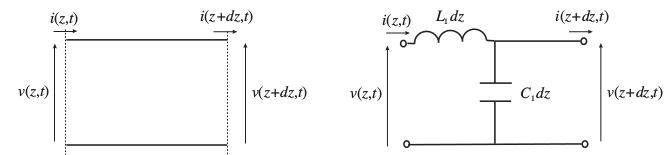
\includegraphics[scale=0.35]{ch2/image4.png}
	\captionof{figure}{ }
\end{wrapfigure}
Il faut procéder à une décomposition infinitésimale car pas d'effet de retard. Considérons 
un tel tronçon. On peut voir un tel tronçon comme une capacité valant $C_1dz$. Comme un courant 
génère un $\vec{B}$, le tronçon captera un flux : apparition d'une inductance par unité de 
longueur
\begin{equation}
L_1 = \dfrac{\phi_1}{i}
\end{equation}
Comme le tronçon est infinitésimal, la théorie des circuit s'applique. Le circuit équivalent 
peut s'écrire mathématiquement
\begin{equation}
\begin{split}
v(z+dz,t) &= v(z,t) - L_1dz\dfrac{\partial i(z,t)}{\partial t}\\
i(z+dz,t) &= i(z,t) - C_1dz\dfrac{\partial v(z,t)}{\partial t}
\end{split}
\end{equation}
où encore\\

\retenir{\ \textbf{équations des télégraphistes}.
\begin{equation}
\begin{split}
\dfrac{\partial v(z,t)}{\partial z} &= -L_1 \dfrac{\partial i(z,t)}{\partial t}\\
\dfrac{\partial i(z,t)}{\partial z} &= -C_1 \dfrac{\partial v(z,t)}{\partial t}
\end{split}
\label{eq:Telegraphistes}
\end{equation}}\ 

Ces équations montre que le courant correspond au courant injecté, diminué du courant de 
fuite dans les capacités. En découplant le système (remplace l'une dans l'autre après 
en avoir dérivée une) en augmentant l'ordre, on retrouve les équations d'ondes
\begin{equation}
\begin{split}
\dfrac{\partial^2 v(z,t)}{\partial z^2} &= L_1C_1\dfrac{\partial^2 v(z,t)}{\partial t^2}\\
\dfrac{\partial^2 i(z,t)}{\partial z^2} &= L_1C_1\dfrac{\partial^2 i(z,t)}{\partial t^2}
\end{split}
\end{equation}
Les tensions et courants se propagent donc à la vitesse 
\begin{equation}
v_p = \dfrac{1}{\sqrt{L_1C_1}}
\end{equation}
On peut écrire, à partir de la définition \autoref{eq:DefZC} de $Z_C$\\
\retenir{\begin{equation}
Z_C = \sqrt{\dfrac{L_1}{C_1}}
\end{equation}}\ \\

\begin{wrapfigure}[9]{r}{4cm}
	\vspace{-5mm}
	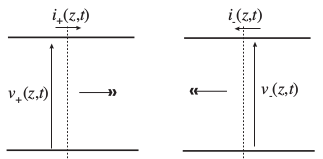
\includegraphics[scale=0.35]{ch2/image5.png}
	\captionof{figure}{Onde progressive (gauche) et régressive (droite)}
\end{wrapfigure}
La solution de ces équations est bien connues : il s'agit d'ondes progressives (droite) ou 
régressives (gauche) se déplaçant à vitesse constante. Le premier type de solution à la 
forme
\begin{equation}
v_+(z,t) = V_+f(t-z/v_p)\qquad V_+\in\mathbb{R}
\end{equation}
où $f$ est une fonction quelconque. Cette solution satisfaisant \autoref{eq:ASat} correspond 
à une tension se propageant le long de la ligne sans atténuation ni déformation. Pour trouver 
le courant $i_+(z,t)$ associé, on utilise
\begin{equation}
\left\{\begin{array}{l}
\autoref{eq:ASat}\\
\autoref{eq:Telegraphistes}
\end{array}\right.\quad\Longrightarrow\quad \dfrac{\partial i_+(z,t)}{\partial t} = 
\dfrac{1}{v_pL_1}\dfrac{\partial v_+(z,t)}{\partial t}
\end{equation}
Après intégration (C.I. nulles)
\begin{equation}
i_+(z,t) = \dfrac{v_+(z,t)}{Z_c}
\end{equation}
Le second type de solution (régressive) est de la forme
\begin{equation}
v_+(z,t) = V_-g(t+z/v_p)\qquad V_-\in\mathbb{R}
\end{equation}
On peut déduire le courant $i_-(z,t)$ (conventionnellement choisi opposé à $i(z,t)$, 
le courant étant défini positif de gauche à droite sur la ligne supérieur) associé à 
cette onde par résolution de l'ED suivante (similairement au cas de l'onde progressive)
\begin{equation}
\dfrac{\partial i_-(z,t)}{\partial t} = -
\dfrac{\partial i(z,t)}{\partial t} = \dfrac{1}{v_pL_1}\dfrac{\partial v_-(z,t)}{\partial t}
\end{equation}
Après intégration
\begin{equation}
i_-(z,t) = \dfrac{v_-(z,t)}{Z_c}
\end{equation}
En fonction de l'écho, nous aurons l'une ou l'autre solution. La tension en un point est 
obtenue en sommant toutes les tensions de toutes les ondes progressives et régressive. Par 
contre, pour le courant, il faut effectuer la différence par convention. A cause de cette 
différence, la tension divisée par le courant ne vaut pas $Z_C$ globalement (mais bien en 
un point)


\section{Réflexions}
	\subsection{Coefficients de réflexion}
	Soit une ligne de transmission sans pertes, uniforme, guidant une onde progressive, 
	de longueur finie $L$. Si $R=Z_C$, la condition sur la tension et le courant à ses 
	bornes s'écrit
	\begin{equation}
	\dfrac{v(L,t)}{i(L,t)} = Z_c
	\end{equation}
	Soit la relation précédemment trouvée : l'onde n'est pas perturbée par la présence de 
	la résistance et pas de formation d'onde réfléchie (entièrement absorbé par la 
	résistance\footnote{"Les charges induites associées à l'onde, "s'écoulent" dans la 
	résistance pour y former un courant"}) : la résistance de charge est \textbf{adaptée}, 
	c'est le cas optimal (rien n'est renvoyé à la source). Si $R\neq Z_c$ 
	\begin{equation}
	\dfrac{v(L,t)}{i(L,t)} = R
	\label{eq:PlusZcMaisR}
	\end{equation}
	Ce qui n'est plus compatible avec \autoref{eq:DefZC} : la quantité de charges induites 
	associée à l'onde ne correspond plus à la valeur du courant exigée par $R$ : perturbation 
	de l'onde et apparition d'une onde réfléchie :
	\begin{equation}
	\begin{array}{ll}
	v(L,t) &= v_+(L,t) + v_-(L,t)\\
	i(L,t) &= i_+(L,t) - i_-(L,t)	= \dfrac{v_+(L,t)}{Z_c}-\dfrac{v_-(L,t)}{Z_c}
	\end{array}
	\end{equation}
	On définit alors $\Gamma_L$, la fraction de l'onde incidente réfléchie : le 
	\textbf{coefficient de réflexion} à la charge
	\begin{equation}
	\Gamma_L = \dfrac{v_-(L,t)}{v_+(L,t)} = \dfrac{i_-(L,t)}{i_+(L,t)}
	\end{equation}
	Avec \autoref{eq:PlusZcMaisR} on trouve\\
	\retenir{\begin{equation}
	\Gamma_L = \dfrac{R-Z_c}{R+Z_c}
	\end{equation}}
	Lorsque la ligne est court-circuitée $R=0 \rightarrow \Gamma_L=-1$ : tension nulle en 
	bout de ligne. Lors que la ligne est ouverte $R=\infty \rightarrow \Gamma = 1$ (courant 
	nul en fin de ligne). L'onde revient à la source et le même phénomène se produit (remplacer 
	$R$ par $R_S$) : nouvelle onde progressive qui se propage !
	
	\subsection{Application}
	Voir page 21-23 : rien de compliqué, ce ne sont que des math. Quelque commentaires sur 
	l'équation (2.30) du syllabus. Le premier terme correspond à un aller, le second au 
	retour, le troisième à un aller-retour, \dots En mettant $\Gamma_L$ en évidence, on fait 
	apparaître une série géométrique. Ces calculs décrivent ainsi un état transitoire : après 
	allumage de la source, on observe plusieurs échos jusqu'à une stabilisation vers le 
	résultat quasi-statique.
	
\section{Les lignes en régime sinusoïdal permanent}
	\subsection{Tension et courant sur la ligne}
	\label{sec:2.5.1}
	Considérons cette fois-ci une source sinusoïdale : légèrement plus compliqué, car tout 
	variera de façon sinusoïdale également (en supposant que la charge en fin de ligne est 
	linéaire).
	\begin{equation}
	v_s(t) = V_S\ \cos(\omega t + \phi_s) = \Re\left(\underline{V}_Se^{j\omega t}\right)
	\end{equation}
	où $V_s$ est l’amplitude de la tension, $\phi_s$ sa phase, $\omega$ sa pulsation et 
	$\underline{V}_S = V_Se^{j\phi_s}$, un phaseur.\\
	On peut faire de même pour les tensions et courants
	\begin{equation}
	\begin{split}
	v(z,t) &= \Re \left(\underline{V}(z)e^{j\omega t}\right)\\
	i(z,t) &= \Re \left(\underline{I}(z)e^{j\omega t}\right)	
	\end{split}
	\end{equation}
	\danger Ces phaseurs dépendent ici de $z$ ! On peut ré-écrire les équations des 
	télégraphistes\\
	\retenir{\begin{equation}
	\begin{split}
	\dfrac{d\underline{V}(z)}{dz} &= -j\omega L_1 \underline{I}(z)\\
	\dfrac{d\underline{I}(z)}{dz} &= -j\omega C_1 \underline{V}(z)	
	\end{split}
	\end{equation}}\ \\
	
	On peut, comme précédemment, découpler le système
	\begin{equation}
	\begin{aligned}
	\dfrac{d^2\underline{V}(z)}{dz^2} &= -\omega^2 L_1C_1\underline{V}(z) &= -\beta^2
	\underline{V}(z)\\
	\dfrac{d^2\underline{I}(z)}{dz^2} &= -\omega^2 L_1C_1\underline{I}(z) &= -\beta^2
	\underline{I}(z)	
	\end{aligned}
	\end{equation}
	où $\beta = \omega\sqrt{L_1C_1}$. La résolution de ces équations donne
	\begin{equation}
	\begin{array}{lll}
	\underline{V}_+(z) = V_+e^{-j\beta z},\qquad\qquad 	\underline{V}_-(z) &= V_-e^{j\beta z}\\
	\underline{I}_+(z) = I_+e^{-j\beta z},\qquad\qquad 	\underline{I}_-(z) &= I_-e^{j\beta z}	
	\end{array}
	\end{equation}
	Nous avons travaillé en phaseur : il s'agit de la situation en régime décrite par la 
	superposition d'une seule onde progressive et une seule onde régressive.
	\begin{equation}
	\begin{array}{ll}
	\underline{V}(z) &= V_+e^{-j\beta z}+V_-e^{j\beta z}\\
	\underline{I}(z) &= I_+e^{-j\beta z}-I_-e^{j\beta z}	
	\end{array}
	\end{equation}
	En utilisant les équations des télégraphistes, on obtient
	\begin{equation}
	\dfrac{V_+}{I_+} = \dfrac{V_-}{I_-} = Z_c
	\end{equation}
	Notons que le terme d'exponentielle imaginaire correspond aux changement de phases dus 
	au délai de propagation. Pour voir une phase constante (argument constant), il faut se 
	déplacer à vitesse
	\begin{equation}
	\dfrac{\omega}{\beta} = \dfrac{1}{\sqrt{L_1C_1}} = v_p
	\end{equation}
	soit la \textbf{vitesse de phase} (qui vaut bien la vitesse de propagation sur la ligne).
	La longueur d'onde, elle, vaut $\lambda = \dfrac{2\pi}{\beta}$.
	
	\newpage
	\subsection{Application}
	Avec $Z_C$, on peut écrire la tension et le courant le long de la ligne
	\begin{equation}
	\begin{split}
	\underline{V}(z) &= V_+e^{-j\beta z} + V_-e^{j\beta z}\\
	\underline{I}(z) &= \dfrac{V_+}{Z_c} e^{-j\beta z} - \dfrac{V_-}{Z_c}e^{j\beta z}	
	\end{split}
	\label{eq:2.45}
	\end{equation}
	En $z=L$
	\begin{equation}
	\dfrac{\underline{V}(L)}{\underline{I}(L)} = Z_L
	\end{equation}
	En définissant le coefficient de réflexion à la charge
	\begin{equation}
	\Gamma_L = \dfrac{\underline{V}_-(L)}{\underline{V}_+(L)} = \dfrac{V_-}{V_+}e^{2j\beta L}
	\label{eq:2.47}
	\end{equation}
	On peut alors écrire la condition en bout de ligne
	\begin{equation}
	Z_L = Z_c\dfrac{1+\Gamma_L}{1-\Gamma_L}\quad\Leftrightarrow\quad \Gamma_L = \dfrac{Z_l-Z_c}{
	Z_l+Z_c}
	\end{equation}
	Les C.I permettent de déterminer $V_+$ et $V_-$. Le calcul ne sera pas détaillé ici. Discutons 
	néanmoins l'expression obtenue
	\begin{equation}
	V_+ = \dfrac{Z_c}{Z_S+Z_c}\left(1+\Gamma_L\Gamma_Se^{-2j\beta L}+\Gamma_L^2\Gamma_S^2e^{-4j\beta L}
	+\dots\right)\underline{V}_S
	\end{equation}
	\begin{wrapfigure}[11]{r}{6.5cm}
	\vspace{-5mm}
	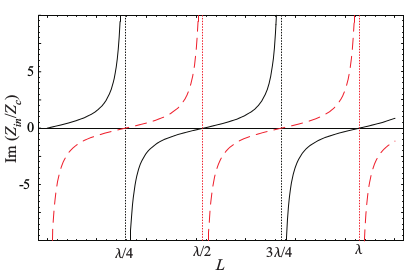
\includegraphics[scale=0.45]{ch2/image6.png}
	\captionof{figure}{ }
	\end{wrapfigure}
	La tension en situation de régime est la superposition de la tension appliquée par la source et de 
	l'ensemble des échos (chaque exp. correspond au délai supplémentaire de chaque écho). Cette 
	expression est intéressante car celle-ci dépend de $L$. Plaçons-nous en $L=\lambda/4$ : la ligne 
	se comporte comme un circuit ouvert. En augmentant $L$, la partie imaginaire devient négative : 
	elle se comporte comme une capacité. On repasse ensuite par $Z=0$, puis on retrouve un comportement 
	inductif. Il s'agit de la courbe pleine ci-contre.\\
	Analysons maintenant la courbe en pointillée correspondant à une ligne \textit{ouverte} (\!!). Si 
	$L=\lambda/4$, le générateur "verra" un circuit fermé ! On voit dès lors qu'à partir d'une ligne, 
	il est possible de réaliser ce que l'on souhaite rien qu'en jouant sur la longueur.
	
	\subsection{Impédance d'entrée}
	L'impédance d'entrée de la ligne est celle vue par la source 
	\begin{equation}
	Z_{in} = \dfrac{\underline{V}(0)}{\underline{I}(0)}
	\end{equation}
	Avec \autoref{eq:2.45} et \autoref{eq:2.47} :
	\begin{equation}
	\begin{split}
	\underline{V}(z) &= V_+\left(e^{-j\beta z} + \Gamma_L e^{-2j\beta L}e^{j\beta z}\right)\\
	\underline{I}(z) &= \dfrac{V_+}{Z_c} \left(e^{-j\beta z} - \Gamma_L e^{-2j\beta L}e^{j\beta z}\right)	
	\end{split}
	\end{equation}
	Par définition de $Z_{in}$\\
	\retenir{\begin{equation}\label{eq:zinzcgammal}
	Z_{in} = Z_c\dfrac{1+\Gamma_L e^{-2j\beta L}}{1-\Gamma_Le^{-2j\beta L}}
	\end{equation}}\ \\
	
	L'impédance d'entrée va non seulement dépendre de l'impédance caractéristique de la ligne connectée, mais également de 
	la longueur de la ligne (un déphasage pouvant causer des interférences est à prendre en compte).
	
	
	\subsection{Ondes stationnaires}
	Nous avons vu que pour bien bosser à HF, il fallait que les éléments soient adaptées pour le 
	traitement des signaux. Or, les composants présentent toujours des tolérances : comment 
	caractériser la désadaptation ? Un outil est le taux d'ondes stationnaires. La tension sur 
	la ligne est la somme d'une onde progressive et régressive (où l'on a utilisé la définition 
	de $V_-$ de la \autoref{sec:2.5.1}) :
	\begin{equation}
	\begin{array}{ll}
	\underline{V}(z) &= V_+(e^{-j\beta z} + \Gamma_L e^{-2j\beta L}e^{j\beta z})\\
	&= V_+e^{-j\beta z}(1+\Gamma_Le^{-2j\beta(L-z)})
	\end{array}
	\end{equation}
	Si la charge est adaptée $\Gamma_L = 0 \rightarrow \underline{V}(z) = V_+e^{-j\beta z}$, 
	soit une seule onde progressive d'amplitude constante $|\underline{V}(z)|=|V_+|$ : en 
	chaque point de la ligne l'oscillation est la même. On remarque bien l'onde progressive 
	dans le temporel (on se simplifie la tâche en supposant $V_+\in\mathbb{R}$)
	\begin{equation}
	v(z,t) = V_+\cos(\omega t-\beta z)
	\end{equation}
	Si la ligne est ouverte $\Gamma_L=1$, on peut faire apparaître un cosinus après mise 
	en évidence :
	\begin{equation}
	\underline{V}(z) = V_+e^{-j\beta z}(1+e^{-2j\beta(L-z)}) = 2V_+e^{-j\beta L}\cos(
	\beta(L-z))\quad\Rightarrow\quad |\underline{V}(z)| = |2V_+\cos(\beta(L-z))|
	\end{equation}
	Ici l'amplitude dépend de la position. En temporel (si $V_+\in\mathbb{R}$)
	\begin{equation}
	v(z,t) = 2V_+\cos(\beta(L-z))\cos(\omega t-\beta L)
	\end{equation}
	Il n 'y a plus de terme de propagation ($\omega t \pm \beta z$) : ceci est une onde 
	stationnaire\footnote{On peut s'en rendre compte en remarquant que les zéros ne 
	dépendent pas de $t$.}. Si on repère des zéros parfait ou des "doublement d'amplitude" 
	parfait c'est que rien n'est absorbé, le récepteur ne fonctionne donc pas.\\
	
	\danger Si la ligne est ouverte mais de longueur $L=\lambda/4 \rightarrow \beta L = 
	\pi/2$ la tension de ligne est nulle et cette ligne apparaît pour la source comme un 
	court-circuit :
	\begin{equation}
	\underline{I}(z) = \dfrac{V_+}{Z_c}e^{)j\beta z}(1-e^{-2j\beta(L-z)}) = \dfrac{2jV_+}{
	Z_c}e^{-j\beta L}\sin(\beta(L-z))
	\end{equation}
	Le courant est bien nul en bout de ligne, mais pas ailleurs : le courant est dû à 
	des oscillations locales et non globales des $e^-$, un courant local peut donc exister. 
	S'il y a du courant, il y a production d'onde EM, c'est le principe de fonctionnement 
	des antennes : un fil suffit car le courant passe même si le fil est ouvert.\\
	
	Étudions maintenant le cas général (tension le long de la ligne en phaseur) :
	\begin{equation}
	\underline{V}(z) = V_+e^{-j\beta z}(1+\Gamma_Le^{-2j\beta(L-z)})\quad\rightarrow\quad
	|\underline{V}(z)| = |V_+||1+\Gamma_Le^{-2j\beta(L-z)}|
	\end{equation}
	Le module de l'imaginaire valant l'unité, l'amplitude varie entre :
	\begin{equation}
	|\underline{V}(z)|_{\max} = |V_+|(1+|\Gamma_L|),\qquad
	|\underline{V}(z)|_{\min} = |V_+|(1-|\Gamma_L|)
	\end{equation}
	Ces deux valeurs ne sont égale que si la charge est adaptée. La désadaptation est 
	alors caractérisée par\\
	\retenir{\textbf{\ VSWR}
	\begin{equation}
	\dfrac{|\underline{V}(z)|_{\max}}{|\underline{V}(z)|_{\min}} = 
	\dfrac{1+|\Gamma_L|}{1-|\Gamma_L|}
	\end{equation}}\ \\
	
	Soit le \textbf{taux d'onde stationnaire en tension}. Plus il est proche de l'unité, 
	mieux c'est. En pratique, on espère $VSWR \leq 2$.
	
	\subsection{Puissance transmise à la charge}
	La puissance moyenne dissipée dans une impédance vaut 
	\begin{equation}
	P = \dfrac{1}{T}\int_0^T v(t)i(t)\ dt\qquad\leftrightarrow\qquad P=\dfrac{1}{2}
	\Re(\underline{V}\underline{I}^*)
	\end{equation}
	La puissance de l'onde progressive et régressive vaudront (on remplace, distribue,\dots) 
	\begin{equation}
	\begin{array}{lll}
	P_+ &= \dfrac{1}{2}	\Re(\underline{V}_+\underline{I}_+^*) &= \dfrac{|V_+|^2}{2Z_c}\\
	P_- &= \dfrac{1}{2}	\Re(\underline{V}_-\underline{I}_-^*) &= \dfrac{|V_-|^2}{2Z_c}	 
	= |\Gamma_L|^2\dfrac{|V_+|^2}{2Z_c}
	\end{array}
	\end{equation}
	où l'on a remplacé $V_-$ par son expression utilisant le coefficient de réflexion.
	Calculons la puissance consommée
	\begin{equation}
	\begin{split}
	P_L &= \dfrac{1}{2}\Re[\underline{V}(L)\underline{I}^*(L)]\\
	&= \Re\left[\dfrac{|V_+|^2}{Z_c}\left(e^{-j\beta L}+\Gamma_Le^{-j\beta L}\right)
	\left(e^{j\beta L}-\Gamma_L^*e^{j\beta L}\right)\right]\\
	&=\Re\left[\dfrac{|V_+|^2}{Z_c}(1-|\Gamma_L|^2) + \dfrac{|V_+|^2}{Z_c}(\Gamma_L-
	\Gamma_L^*)\right]
	\end{split}
	\end{equation}
	Comme $\Gamma_L-\Gamma_L^*$ est purement imaginaire :
	\begin{equation}
	P_L = \dfrac{1}{2}\dfrac{|V_+|^2}{Z_c}(1-|\Gamma_L|^2) = P_+-P_-
	\end{equation}
	Ce que l'utilisateur "utilise" est bien la différence entre ce qui est injecté et 
	réfléchi. Conventionnellement on fixe $\Gamma_L=1/3$ pour avoir une puissance 
	transmise de 90\%.
	
	\subsection{Les pertes}
	\begin{wrapfigure}[6]{r}{6.5cm}
	\vspace{-7mm}
	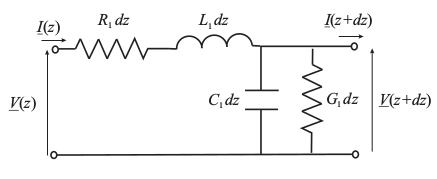
\includegraphics[scale=0.45]{ch2/image7.png}
	\captionof{figure}{ }
	\end{wrapfigure}
	IRL, il y a toujours des pertes (joules dans les fils et dans les diélectriques 
	(ils chauffent, effet four à micro-onde)). 
	Modélisons les pertes joues par une résistance linéaire $R_1$ et les pertes 
	diélectriques par une conductance linéique $G_1$ en parallèle. Les équations des 
	télégraphistes s'écrivent
	\begin{equation}
	\begin{split}
	\dfrac{d\underline{V}(z)}{dz} &= -(R_1+j\omega L_1)\underline{I}(z)\\
	\dfrac{d\underline{I}(z)}{dz} &= -(G_1+j\omega C_1)\underline{V}(z)	
	\end{split}
	\end{equation}
	En découplant
	\begin{equation}
	\begin{aligned}
	\dfrac{d^2\underline{V}(z)}{dz^2} &= (R_1+j\omega L_1)(G_1+j\omega C_1)\underline{V}(z)
	&= \gamma^2\underline{V}(z)\\
	\dfrac{d^2\underline{I}(z)}{dz^2} &= (R_1+j\omega L_1)(G_1+j\omega C_1)\underline{I}(z)
	&= \gamma^2\underline{I}(z)	
	\end{aligned}
	\end{equation}
	où $\gamma = \alpha+j\beta= \sqrt{(R_1+j\omega L_1)(G_1+j\omega C_1)}$, la constante de 
	propagation complexe. Les solutions de la première équations sont
	\begin{equation}
	\begin{array}{lllll}
	\underline{V}_+(z) &= V_+e^{-\gamma z} &= V_+e^{-\alpha z}e^{-j\beta z} \quad &\rightarrow
	\quad v_+(z,t) &= 	V_+e^{-\alpha z}\cos(\omega t-\beta z)\\
	\underline{V}_-(z) &= V_-e^{\gamma z} &= V_-e^{\alpha z}e^{j\beta z}  \quad &\rightarrow
	\quad v_-(z,t) &= 	V_-e^{\alpha z}\cos(\omega t+\beta z)	
	\end{array}
	\end{equation}
	Les pertes causent une atténuation exponentielle du signal. Pour l'onde régressive, on 
	pourrait croire que l'exponentielle positive n'est pas physique mais il n'en n'est rien : 
	les $z$ décroissent. On retrouve des solution semblables pour le courant
	\begin{equation}
	\begin{array}{ll}
	\underline{I}_+(z) &= I_+e^{-\gamma z}\\
	\underline{I}_-(z) &= I_-e^{\gamma z}	
	\end{array}
	\end{equation}
	Selon les équations des télégraphistes $\displaystyle \dfrac{V_+}{I_+}=\dfrac{V_-}{I_-}=Z_c$, 
	désormais $Z_c\in\mathbb{C}$ :
	\begin{equation}
	Z_c=\sqrt{\dfrac{R_1+j\omega L_1}{G_1+j\omega C_1}}
	\end{equation}
	La puissance de l'onde progressive vaut, à l'aide de la précédente sous-section :
	\begin{equation}
	P_+(z) = \Re\left(\dfrac{|V_+|^2}{2Z_c^*}\right)e^{-2\alpha z}
	\end{equation}
	où $\alpha$ est bien la partie réelle de la constante de propagation : cette constante 
	est à connaître. Hélas, elle n'est jamais directement donnée (trop facile). On peut 
	néanmoins la retrouver avec
	\begin{equation}
	\alpha_d[\si{\decibel}] = 10\log\dfrac{\Re\left(\dfrac{|V_+|^2}{2Z_c^*}\right)e^{-2\alpha z}}{
	\Re\left(\dfrac{|V_+|^2}{2Z_c^*}\right)e^{-2\alpha (z+d)}} = 20\log e^{\alpha d} = 
	(20\log e)\alpha d = 8,686\alpha d
	\end{equation}
	où $d$ est une distance.
	
	
\section{Scattering parameters}

	\begin{wrapfigure}[7]{l}{5.15cm}
	\vspace{-5mm}
	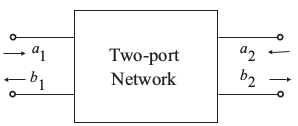
\includegraphics[scale=0.45]{ch2/image8.png}
	\captionof{figure}{ }
	\end{wrapfigure}
Considérons un quadripôle. Nous allons essayer de trouver une matrice de transformation entre 
l'entrée et la sortie, non plus en terme de tension mais en terme d'onde progressive et 
régressive. Il s'agit d'une théorie complexe mais assez simple dans le cas ou $Z_c\in\mathbb{R}$.\\
Afin d'éliminer les $Z_c$, définissons les paramètres (d'entrée ($a)$ et de sortie $(b)$ des 
entrées 1 et 2) :
\begin{equation}
\begin{aligned}
a_1 &= \dfrac{V_{1+}}{\sqrt{Z_c}},\quad a_2 &= \dfrac{V_{2+}}{\sqrt{Z_c}}\\
b_1 &= \dfrac{V_{1-}}{\sqrt{Z_c}},\quad b_2 &= \dfrac{V_{2-}}{\sqrt{Z_c}}
\end{aligned}
\end{equation}
La \textbf{matrice de répartition} (\textit{scattering matrix}) permet de lier la sortie 
à l'entrée
\begin{equation}
\left(\begin{array}{c}
b_1\\
b_2
\end{array}\right) = \left(\begin{array}{cc}
S_{11} & S_{12}\\
S_{21} & S_{22}
\end{array}\right)\left(\begin{array}{c}
a_1\\
a_2
\end{array}\right)
\end{equation}
La mesure des $S-$paramètres ne nécessite que la connaissance de l'impédance des ports. Par 
exemple, pour $S_{11}$ :
\begin{equation}
S_{11} = \left.\dfrac{b_1}{a_1}\right|_{a_2=0}
\end{equation}
	
	
\section{The Smith Chart}
	\begin{wrapfigure}[9]{l}{5.15cm}
	\vspace{-5mm}
	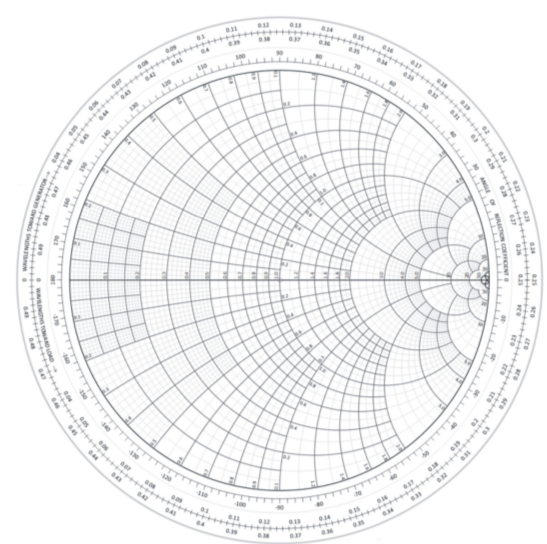
\includegraphics[scale=0.25]{ch2/image9.png}
	\captionof{figure}{ }
	\end{wrapfigure}
L'abaque de Smith est historiquement important : il était utilisé avant l'arrivée de Matlab 
et ses srabs. Nous avions vu que le coefficient de réflexion en \textbf{bout de ligne} était 
donné par
\begin{equation}
\Gamma(L) = \dfrac{Z_L-Z_c}{Z_L+Z_c}
\end{equation}
Connaissant les phaseurs des ondes progressives et régressives, on peut obtenir une expression 
donnant le coefficient de réflexion en chaque point
\begin{equation}
\Gamma(z) = \dfrac{\underline{V}_-(z)}{\underline{V}_+(z)}=\Gamma(L)e^{2j\beta(z-L)} 
\end{equation}
où $\beta = \omega\sqrt{L_1C_1}$. On peut encore écrire cette expression avec celle de l'impédance 
d'entrée
\begin{equation}
\Gamma(z) = \dfrac{Z_{in}(z)-Z_c}{Z_{in}(z)+Z_c}
\end{equation}
où $Z_{in}(z) = Z_c\dfrac{1+\Gamma(z)}{1-\Gamma(z)}$. On peut définir une impédance d'entrée 
normalisée $z_{in} = r+jx = Z_{in}(z)/Z_c$. En écrivant
\begin{equation}
\Gamma(z) = \Gamma_r + j\Gamma_i
\end{equation}
Avec cette décomposition et celle de $z_{in}$, on peut écrire
\begin{equation}
r+jx = \dfrac{1+\Gamma_r+j\Gamma_i}{1-\Gamma_r-j\Gamma_i} = \dfrac{1-\Gamma_r^2-\Gamma_i^2+2j
\Gamma_i}{(1-\Gamma_r)^2+\Gamma_i^2}
\end{equation}
En identifiant $r$ et $x$, on peut obtenir deux équations de cercles après réarrangement :
\begin{equation}
\begin{split}
\left(\Gamma_r -\dfrac{r}{r+1}\right)^2 + \Gamma_i^2 &= \left(\dfrac{1}{1+r}\right)^2\\
(\Gamma_r-1)^2 +\left(\Gamma_i-\dfrac{1}{x}\right)^2 &= \left(\dfrac{1}{x}\right)^2
\end{split}
\end{equation}
On obtient ainsi un ensemble de cercles $r$ et $x$ constant. En les superposant et en 
choisissant un point $x$ et $r$, il est possible de trouver $\Gamma_i$ et $\Gamma_r$. C'est 
un bazooka pour quelque chose d'assez simple, mais il faut au moins en avoir entendu 
parlé une fois.

\section{Impedance matching}
Il est important que l'impédance de charge soit adaptée par rapport à l'impédance caractéristique de ligne, c-à-d $Z_L=Z_c$. Si ce n'est pas le cas, il faut insérer dans le circuit un adaptateur d'antenne (matching network) comme représenté \autoref{fig:MatchNet}. Supposons qu'on ait des lignes de transmission sans pertes, ceci permettant de considérer $Z_c\in\mathbb{R}$.\\

On utilise un adaptateur d'antenne afin de satisfaire $Z_{in} = Z_c$. Dans la plupart des cas, $Z_L\in\mathbb{C}$, l'adaptateur doit donc fixer 2 degrés de liberté ($\Re$ et $\Im$). On va en parler de 2, le \emph{transformateur quart d'onde} pour le cas où $Z_L\in\mathbb{R}$, l'\emph{embout d'adaptation} (stub matching) pour le cas général.
\subsection{Transformateur quart d'onde}
Hypothèse: $R_L\in\mathbb{R}$. Représente \autoref{fig:transfoquartonde}, il consiste à rajouter une ligne de transmission sans perte de longueur $L=\lambda/4$ et d'impédance caractéristique $Z_{qw}\neq Z_c$. À l'aide de \eqref{eq:zinzcgammal} 
\begin{equation}
	Z_{in}= Z_{qw}\frac{1+\Gamma_L e^{-2j\beta L}}{1-\Gamma_L e^{-2j\beta L}}
\end{equation}
avec $L=\lambda/$ et $\Gamma_L=\frac{R_L-Z_{qw}}{R_L+Z_{qw}}$, donc
\begin{equation}
	Z_{in}=\frac{Z_{qw}^2}{R_L}
\end{equation}
$\Rightarrow Z_{in}\in\mathbb{R}$.  Pour avoir $Z_{in}=Z_c$
\begin{equation}
	Z_{qw} = \sqrt{Z_c R_L}
\end{equation}
\subsection{Embout d'adaptation}
Si $R_L\in\mathbb{C}\Rightarrow$ 2 degré de liberté. Ici, on va placer à une distance $d$ de $R_L$ une réactance $Y_s$ en parallèle avec la ligne (degré de liberté: $d$ et $Y_s$) comme représenté \autoref{fig:emboutadap}. Comme la réactance est en parallèle avec la ligne, $Y_c=1/Z_c$.\\

On commence sans la réactance en parallèle. La réactance d'entrée vue à une distance $d$ de la charge est donnée par l'inverse de \eqref{eq:zinzcgammal} avec $z=L-d$
\begin{equation}
	Y_{in}=Y_c \frac{1-\Gamma(L-d)}{1+\Gamma(L-d)}
\end{equation}
On sait toujours choisir $d$ tel que $\Re(Y_{in})=Y_c$. $Y_{in}$ prend donc la forme suivante
\begin{equation}
	Y_{in} = Y_c+jB
\end{equation}
Maintenant, on ajoute la réactance $Y_s$ en parallèle au point $d$. La réactance d'entrée totale devient
\begin{equation}
	Y_{in} = Y_c + jB+ Y_s
\end{equation}
on est adapté lorsque $Y_s = -jB$. En pratique, la réactance est définie sur base de test avec un embout circuit-ouvert ou un embout court-circuit d'une ligne de transmission sans perte.
\begin{figure}[H] 
	\centering
	\subfigure[Adaptation d'antenne]{\label{fig:MatchNet}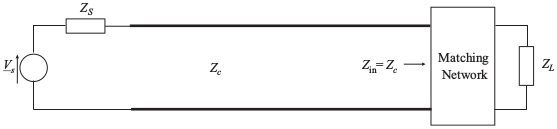
\includegraphics[width=.8\textwidth]{ch2/image10}}
	\subfigure[Transformateur quart d'onde]{\label{fig:transfoquartonde}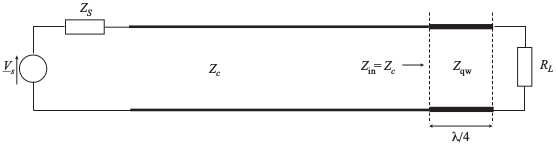
\includegraphics[width=.8\textwidth]{ch2/image11}}
	\subfigure[Embout d'adaptation]{\label{fig:emboutadap}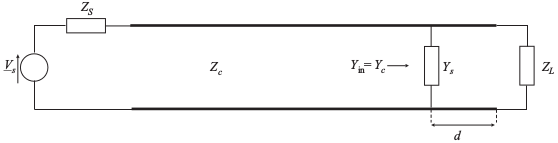
\includegraphics[width=.8\textwidth]{ch2/image12}}
	\caption{Adaptation d'antenne} 
\end{figure}
	
	
	
	
	
	
	
	
	
	
	
	
	
	
	
	
	



